\documentclass[xcolor=dvipsnames, 11pt]{beamer}

\usetheme{Warsaw}

\usepackage{ucs}
\usepackage[utf8x]{inputenc}
\usepackage[greek,english]{babel}
\usepackage{hyperref}
\usepackage{tcolorbox}
\usepackage{alphabeta}
\usepackage{amsmath}
\usepackage{amsthm}
\usepackage{caption}

\tcbuselibrary{theorems}

\newtcbtheorem{mytheorem}{\el Ορισμός}%
{colback=blue!5,colframe=black!15!black,fonttitle=\bfseries}{th}

\newtcbtheorem{mytheor}{\el Θεώρημα}%
{colback=blue!5,colframe=black!15!black,fonttitle=\bfseries}{th}

\newcommand{\en}{\selectlanguage{english}}
\newcommand{\el}{\selectlanguage{greek}}

\setbeamertemplate{itemize items}[ball]
\setbeamertemplate{itemize subitem}[ball]

\begin{document}

\title{Travelling Salesman Problem}
\subtitle{TSP}

\author[\el Σιώρος Βασίλειος, Ανδρινοπούλου Χριστίνα]{\el Σιώρος Βασίλειος \and \el Ανδρινοπούλου Χριστίνα}
\date{\el Απρίλιος, 2020}

\frame{\titlepage}

\begin{frame}
	\frametitle{\el Θεωρητική Προσέγγιση}
	\begin{itemize}
		\item \el Γραφοθεωρητική προσέγγιση
		\begin{itemize}
			\item \el Tο \en TSP \el είναι μία επέκταση του προβλήματος εύρεσης κυκλώματος \en Hamilton.
		\end{itemize}
		\item \el Γεωμετρική προσέγγιση
		\begin{itemize}
			\item \en Delaunay \el τριγωνοποίηση
			\begin{itemize}
				\item \el Προσεγγιστική εύρεση μονοπατιου 
				\item \el Αλγόριθμος εύρεσης μονοπατιού
			\end{itemize} 
			\item \en Time Window TSP \el και \en Time Window Prize Collecting
			\begin{itemize}
				\item \en 1D
				\item \en Metric Space
			\end{itemize}
			\item \en Universal TSP
		\end{itemize}
	\end{itemize}
\end{frame}

\begin{frame}
	\frametitle{\el Υλοποίηση}
	\begin{columns}[t]
		\column{.4\textwidth}
		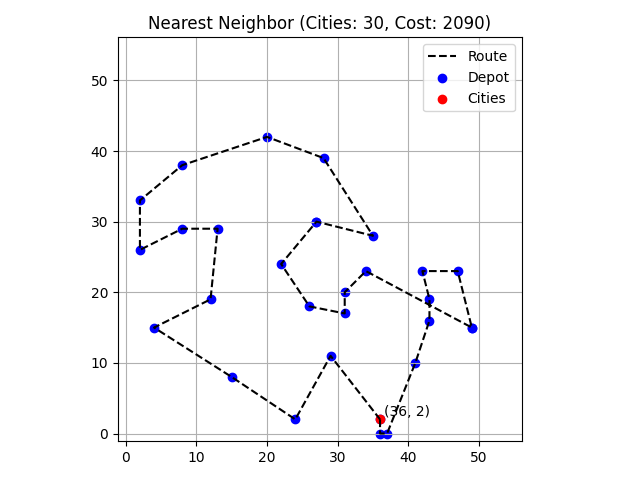
\includegraphics[width=\columnwidth,height=2.8cm]{images/nearest_neighbor_030_2090.png}
		\captionof{figure}{Nearest neighbor με Ευκλείδια μετρική}
		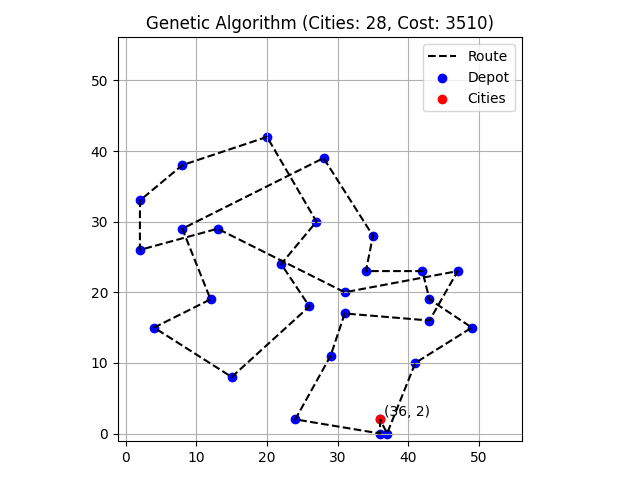
\includegraphics[width=\columnwidth,height=2.8cm]{images/genetic_algorithm_028_3510.png}
		\captionof{figure}{Opt-2 με Ευκλείδια μετρική}
		\column{.4\textwidth}
		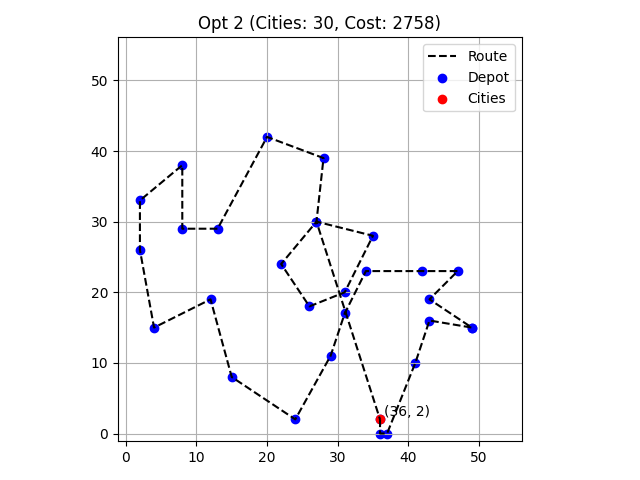
\includegraphics[width=\columnwidth,height=2.8cm]{images/opt_2_030_2758.png}
		\captionof{figure}{Genetic Algorithm με Ευκλείδια μετρική}
		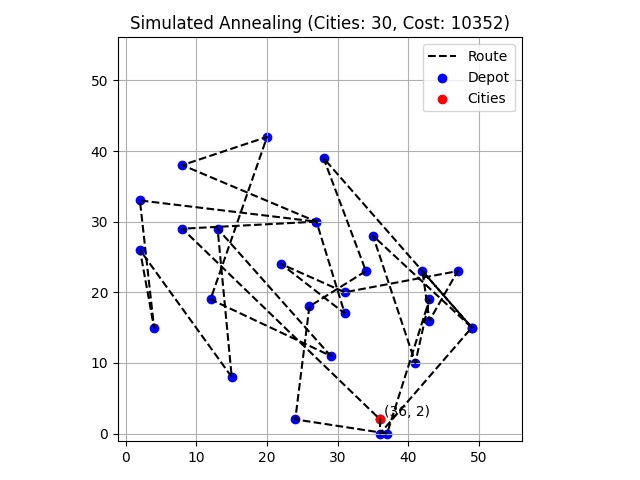
\includegraphics[width=\columnwidth,height=2.8cm]{images/simulated_annealing_030_10352.png}
		\captionof{figure}{Simulated Annealing με Ευκλείδια μετρική}
	\end{columns}
\end{frame}

\begin{frame}
	\frametitle{\el Υλοποίηση}
	\begin{columns}[t]
		\column{.6\textwidth}
		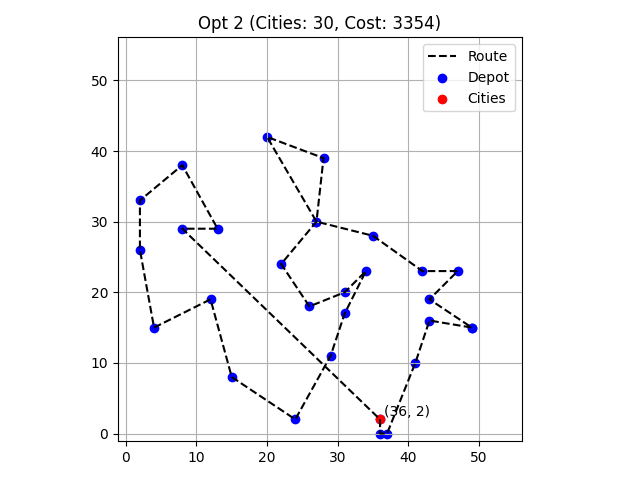
\includegraphics[width=\columnwidth,height=4cm]{images/combo_annealing_opt.png}
		\captionof{figure}{Simulated Annealing \(\rightarrow\) Opt-2}
		\column{.6\textwidth}
		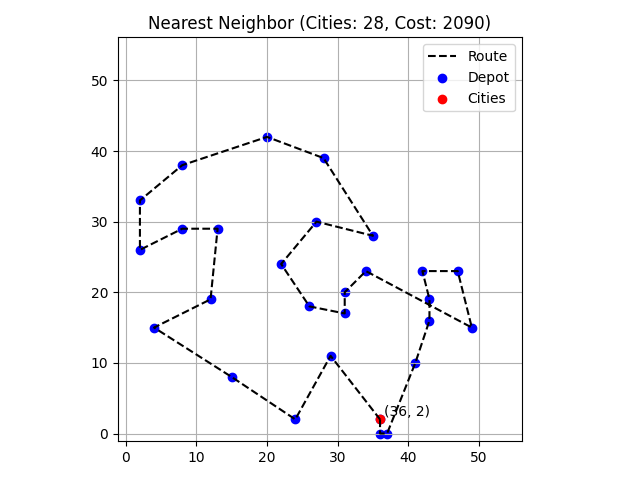
\includegraphics[width=\columnwidth,height=4cm]{images/combo_genetic_neighbor.png}
		\captionof{figure}{Genetic Algorithm \(\rightarrow\) Nearest Neighbor}
	\end{columns}
\end{frame}


\begin{frame}
	\frametitle{References}
	\begin{itemize}
		\item \textit{\en Exact and Approximation Algorithms for Time-Window TSP, 
			Jie Gao, Su Jia, Joseph S. B. Mitchell,
			CG:YRF, Boston, MA, USA, June 14-18, 2016}
		\item \textit{\en An Optimal Lower Bound for the Hilbert-type, Planar Universal Traveling Salesman Problem, Patrick Eades, Julián Mestre,	CG:YRF, Brisbane, Australia, July 4-7, 2017}
		\item \textit{\en An O ( n log n ) Heuristic for the Euclidean Traveling Salesman Problem, 
			Evgeny Yanenko, Eckart
		Schuhmacher, Ulrich Spörlein, Kurt Tutschku,	April 25, 2005}
		\item \textit{Approximation Algorithms for Time-Window TSP and Prize Collecting TSP Problems,
			Jie Gao, Su Jia, Joseph S. B. Mitchell, Lu Zhao,
			Stony Brook University, Stony Brook, NY 11794, USA.}
		\item \text{\en Applications of the TSP,} \\
		\text{http://www.math.uwaterloo.ca/tsp/apps/index.html}	
\end{itemize}
\end{frame}

\begin{frame}
	\frametitle{References}
	\begin{itemize}
		\item \textit{\el Εισαγωγή στους αλγορίθμους, Δεύτερη έκδοση, \en Thomas H. Cormen, Charles E. Leiserson, Ronald L. Rivest, Clifford Stein, \el Πανεπιστημιακές εκδόσεις Κρήτης, 2011, \en ISBN: 978-960-524-473-6}
		\item \textit{\el Τεχνητή Νοημοσύνη, Μία σύγχρονη προσέγγιση, Δεύτερη Αμερικανική έκδοση, \en Stuart Russel, Peter Norvig, \el σελ.: 101,	Κλειδάριθμος 2005, \en ISBN: 960-209-873-2}
		\item \textit{\el Στοιχεία διακριτών μαθηματικών, \en C. L. Liu, \el σελ.: 171-172, 178-179, 190-201, Πανεπιστημιακές εκδόσεις Κρήτης 2014, \en ISBN: 978-960-524-072-1}	
	\end{itemize}
\end{frame}

\begin{frame}
	\frametitle{References}
	\begin{itemize}
		\item \textit{\en Discrete and Computational Geometry, Satyan L. Devadoss, Joseph O'Rourke,
			\el σελ.: 81-86, \en Princeton University Press, 2011, ISBN: 978-0-691-14553-2}
		\item \textit{\en Computational Geometry,	Algorithms and Applications, Third Edition, 
			Mark de Berg, Otfried Cheong, Marc van Kreveld, Mark Overmars, \el σελ.: 193-204,
			\en Springer, 2008, ISBN: 978-3-540-77973-5}
		\item \textit{\el Υπολογιστική Γεωμετρία: Μια σύγχρονη αλγοριθμική προσέγγιση, Γιάννης Ζ. Εμίρης,
			σελ.: 199-208, Κλειδάριθμος, 2008, \en ISBN: 978-960-461-141-6 }	
	\end{itemize}
\end{frame}

\end{document}